\documentclass[times, 12pt, utf8]{article}
\RequirePackage[utf8]{inputenc}
\RequirePackage[croatian]{babel}

\usepackage{listings, lstautogobble}
\usepackage{hyperref, url}
\usepackage{enumitem}
\usepackage{titlesec}
\usepackage{graphics}
\usepackage{graphicx}
\usepackage{xcolor}

% image location
\graphicspath{ {../misc/} }

% xcolor configuration
\definecolor{darkBlue}{HTML}{171f68}

% hyperref configuration
\hypersetup{
	colorlinks=true,
	linkcolor=black,
	filecolor=magenta,      
	urlcolor=darkBlue
}

% code block settings
\lstset { %
	language=C++,
	basicstyle=\ttfamily,
	keywordstyle=\color{blue}\ttfamily,
	stringstyle=\color{red}\ttfamily,
	commentstyle=\color{green}\ttfamily,
	morecomment=[l][\color{magenta}]{\#},
	autogobble=true,
	backgroundcolor=\color{gray!5},
	frame=single,
	framexrightmargin=15pt
}

% titlesec configuration
\titleformat{\section}{
	\normalfont\Large\bfseries
}{\thesection}{1em}{}

\titleformat{\subsection}{
	\normalfont\large\bfseries\raggedright
}{}{0em}{\underline}[]

\begin{document}
	
	\begin{titlepage}
		\clearpage
		\thispagestyle{empty}
		\pagenumbering{gobble}
		
		\title{
			{\large Projekt iz programske potpore} \\
			{ \textbf{Bioinformatika - Poravnavnaje i mapiranje sekvenci genoma} }
			
			\vbox{}
			\vspace{0.5cm}
			
			\footnotesize{
				\begin{itemize}[leftmargin=3.5cm]
					\setlength{\itemindent}{0.8cm}
					
					Voditelji: 
					\item[-] Prof. dr. sc. Mile Šikić
					\item[-] Mag. ing. Robert Vaser
				\end{itemize}
				
			}
			
			\date{}
		}
		
		\clearpage
	\end{titlepage}
	
	\maketitle
	
	\newpage
	\clearpage
	\pagenumbering{gobble}
	
	\tableofcontents
	
	\newpage
	\clearpage
	\pagenumbering{arabic}
	
	\section{Uvod}
	U sklopu predmeta 'Projekt iz programske potpore' na Sveučilištu u Zagrebu,
	Fakultet elektrotehnike i računarstva, studenti u međusobnoj suradnji 
	pod nadzorom profesora i asistenata rješavaju praktične probleme
	s ciljem upoznavanja alata i tehnika korištenih u struci. Grupa 
	okupljena pod vodstvom prof. dr. sc. Mile Šikića bavi se 
	poravnavanjem i mapiranja genoma koristeći moderni C++,
	sustav za upravljene izvornim kodom (eng. version control) git,
	automatizirani sustav izgradnje (eng. build system) CMake,
	sustav kontinuirane integracije TravisCI.
	Po završetku projekta, studenti bi trebali stječi vještine 
	korištenja spomenutih tehnologija te ujedno biti u stanju 
	implementirati osnovne algoritme iz područja bioinformatike.
	
	\section{Rad na projektu}
	
	Prije početka rada na projektu, studenti su dužni proći 
	navedene lekcije ako nisu upoznati sa zadanim tehnologijama: 
	\\ \indent 
	\href
	{http://www.cplusplus.com/doc/tutorial/}
	{C++}
	, \href
	{http://rogerdudler.github.io/git-guide/}
	{GitHub}
	, \href 
	{https://cmake.org/cmake-tutorial/}
	{CMake}
	, \href
	{https://github.com/google/googletest/blob/master/googletest/docs/primer.md}
	{GoogleTest}
	, \href
	{https://docs.travis-ci.com/user/getting-started/}
	{TravisCI} \\ \\
	Također, poželjno je pridržavati se 
	\href {https://google.github.io/styleguide/cppguide.html}{Googleovih smjernica}
	za pisanje i oblikovanje C++ koda.
	Po početku rada studenti su podjelljeni u timove: blue, orange, pink i brown.
	\footnote{\href {https://en.wikipedia.org/wiki/Reservoir_Dogs}{White?}}
	Svaki tim ima svoju git granu i dozvoljeno je kreiranje novih s imanovanjem 
	formata: \colorbox{gray!30}{'white\_feature\_one'}.
	
	\subsubsection{Cilj}
	Studenti će implementirati biblioteku koja podržava nekoliko algoritama
	za mapiranje velikog broja relativno malih podnizova znakova na veliki 
	niz znakova koji predstavlja referentni genom. Cilj je povezati
	implementirane biblioteke u jedan program, obično nazvan eng. mapper, 
	s ciljem poravnanja skeniranih sekvenci.
	
	\begin{figure}[h]
		\centering
		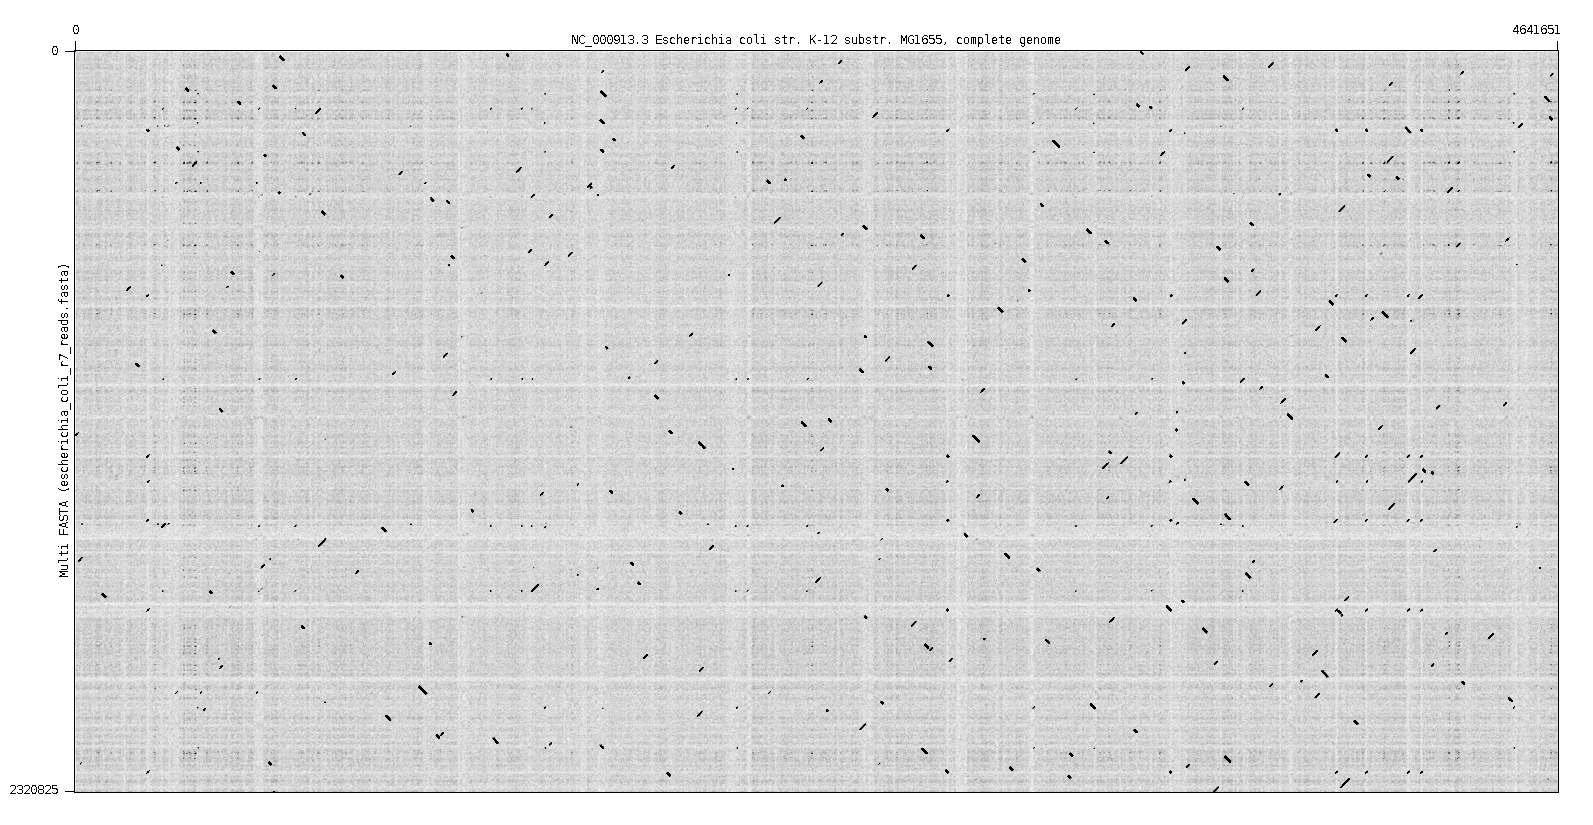
\includegraphics[width=\textwidth]{sample_mappings.png}
		\caption{Vizualni prikaz}
	\end{figure}
	
	\subsection{Zadaci}
	\subsubsection{Alati, okruženje, učitavanje podataka}
	Svaki tim dužan je držati README.md svoje grane usklađenim 
	s README.md glavne (eng. master) grane. Kao uvod u projekt,
	svaki tim treba postaviti strukturu projekta i inicijalizirati
	CMake postavke za izgradnju glavnog programa s imenom formata 
	\colorbox{gray!30}{$<$ime tima$>$\_mapper} (npr. \colorbox{gray!30}{white\_mapper})
	Program preko naredbene konzole mora prihvatiti dva argumenta:
	put do skeniranih sekvenci i put do referentnog genoma.
	Skenirane sekvence trebaju biti u  
	\href
	{hhttps://en.wikipedia.org/wiki/FASTA_format}
	{FASTA} ili
	\href
	{https://en.wikipedia.org/wiki/FASTQ_format}
	{FASTQ} formatu, a referentni genom je
	isključivo podržan u 
	\href
	{hhttps://en.wikipedia.org/wiki/FASTA_format}
	{FASTA} formatu.
	Povodom učitavanja podataka i njihovog spremanja u memoriju, 
	potrebno je ispisati određene statistike na \colorbox{gray!30}{stderr}
	(duljina najkraće i najdulje sekvence, prosječna duljina sekvence...) 
	Studenti nisu dužni samostalno implementirati parser za navedene
	tipove podataka već se mogu koristiti gotovim rješenjem 
	\href {https://github.com/rvaser/bioparser}{bioparser} dodajući ga
	u svoj projekt putem git submodula i CMake, ali moraju provjeriti 
	jesu li ekstenzije predanih datoteka podržane (
	\colorbox{gray!30}{.fasta}
	\colorbox{gray!30}{.fa}
	\colorbox{gray!30}{.fastq}
	\colorbox{gray!30}{.fq}
	\colorbox{gray!30}{.fasta.gz}
	\colorbox{gray!30}{.fa.gz}
	\colorbox{gray!30}{.fastq.gz}
	\colorbox{gray!30}{.fq.gz}
	)
	
	\subsubsection{Poravnanaje sekvenci}
	Cilj ovog podzadatka je implementirati razne algoritme 
	bazirane na dinamičkom programiranju za poravnavanje 
	nizova genoma kako bi se ustvrdila njihova sličnost. 
	Ona se temelji na broju transformacija potrebnih za pretvaranje 
	jednog niza u drugi. Generalni koncept udaljenosti
	uređivanja (eng. edit distance) detaljnije je objašnjen na
	\href {https://en.wikipedia.org/wiki/Edit_distance}{Wikipediji} 
	i u knjizi \href
	{https://www.fer.unizg.hr/_download/repository/bioinformatika_skripta_v1.2.pdf}
	{FER - Bioinformatika}
	
	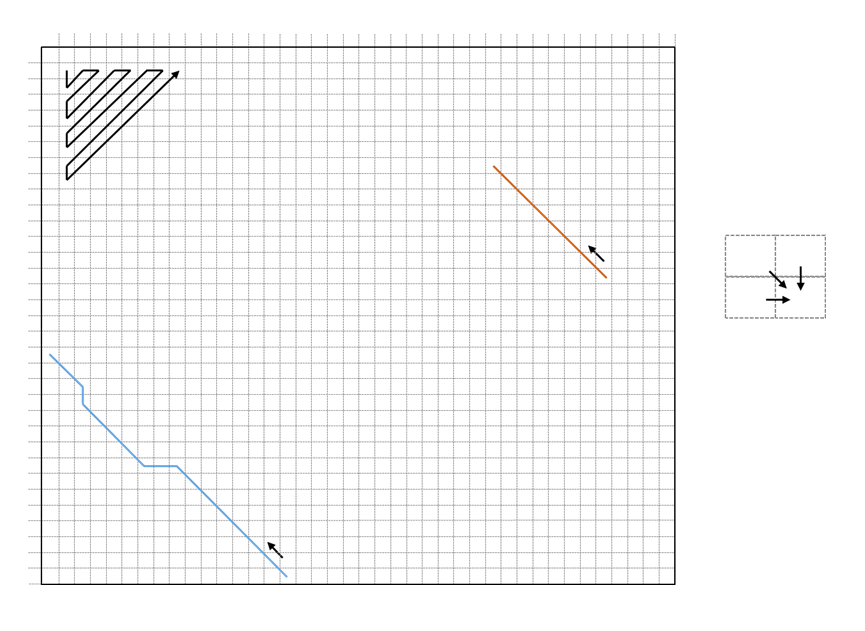
\includegraphics[width=\textwidth]{sample_alignment.png} 
	
	Zadani algoritmi:
	\begin{itemize}
		\item[--] \href
		{https://en.wikipedia.org/wiki/Needleman–Wunsch_algorithm}
		{Needleman-Wunsch} za globalno poravnanje
		\item[--] \href
		{https://en.wikipedia.org/wiki/Smith–Waterman_algorithm}
		{Smith-Waterman} za lokalno poravnanje 
		\item[--] Sufiks/prefiks derivati Needleman-Wunsch algoritma 
		za polu-globalno poravnanje. Detaljnije u   
		\href
		{https://www.fer.unizg.hr/_download/repository/bioinformatika_skripta_v1.2.pdf}
		{FER - Bioinformatika}
	\end{itemize}
	
	Sve implementacije trebaju biti sadržane unutar namespacea jedne biblioteke, 
	s nazivom formata \colorbox{gray!30}{$<$ime tima$>$\_alignment} 
	(npr. \colorbox{gray!30}{white\_alignment}). Bibiloteka
	treba sadržavati dvije funkcije s navedenim prototipima:
	
	\begin{lstlisting}
	int pairwise_alignment(
	const char* query, unsigned int query_length,
	const char* target, unsigned int target_length, 
	AlignmentType type,
	int match,
	int mismatch,
	int gap);
	\end{lstlisting}
	
	\begin{lstlisting}
	int pairwise_alignment(
	const char* query, unsigned int query_length,
	const char* target, unsigned int target_length, 
	AlignmentType type,
	int match,
	int mismatch,
	int gap);
	\end{lstlisting}
	
	Drugi prototip funkcije prima dodatna dva argumenta preko kojih
	vraća početak poravnanja unutar \colorbox{gray!30}{target}
	sekvence i odgovarajući \href {https://samtools.github.io/hts-specs/SAMv1.pdf}{CIGAR} string.
	
	\subsubsection{DNA Minimizeri}
	\subsubsection{Mapiranje sekvenci}
	Posljednji zadatak bio je poravnati ulazne fragmente s danim referentnim genomom.
	Nakon kreiranja indeksa minimizera iz referentnog genoma i uklanjanja f najčešćih minimizera, za svaki fragment zasebno pronalaze se poklapanja minimizera fragmenta i referentnog genoma. Iz liste poklapanja, najduži lanac najbolji je kandidat za dobro poravnanje. Tu regiju (lanac) najlakše je pronaći rješavanjem problema najdužeg rastućeg podniza (eng. \href{https://en.wikipedia.org/wiki/Longest_increasing_subsequence}{longest increasing subsequence problem}) nad listom minimizera koji se poklapaju. 
	Potom se nad pronađenim regijama može pozvati procedura poravnavanja. \\
	Maper ispisuje pronađene regije u \href{https://github.com/lh3/miniasm/blob/master/PAF.md}{PAF} formatu. Ako je argument \colorbox{gray!30}{c} pozvan u naredbenom retku, potrebno je u ispis dodati i CIGAR string.
	Dodatno, argumentom \colorbox{gray!30}{t} unosi se broj dretvi koje maper koristi. Za ovaj dio zadatka studenti mogu koristiti \href{https://www.openmp.org/}{OpenMP} ili \href{https://github.com/rvaser/thread_pool}{thread\_pool}.
	
	\subsection{Rezultati}
	
	\section{Literatura}
	
	\begin{itemize}
		\item[--] \href
		{https://www.fer.unizg.hr/_download/repository/bioinformatika_skripta_v1.2.pdf}
		{FER - Bioinformatika}
	\end{itemize}
	
\end{document}